% METHOD
%=============================================================================
% Light curve simulations
%   - Intro
%   - Planet injections
%   - Planet detection
%   - Optimizing cadence and observing strategy
% Results
%   - Prospects: yields and predictions
% Discussion & Conclusion
%   - Caveats and challenges
%   - Implications
%=============================================================================

\section{Method}

% Light curve simulations - Intro
We tested the potential for finding extra-galactic planets and small stars in
this survey by simulating light curves with a cadence of five minutes and a
white noise amplitude of 5.3\%, estimated using the DECam exposure time
calculator.
We assumed that observations would take place continuously over 6 hours per
night, for 9 nights.
% We also used these simulations to optimize our observing strategy.
%   - Planet injections
We generated transit signals for planets with a range of randomly generated
radii and orbital periods, all orbiting Sun-like stars.
The orbital periods of these planets ranged from around 8 hours to 10 days and
the planet sizes ranged from 0.5 to 2 times the radius of Jupiter.
2000 Exoplanet transit signals were generated using the {\tt batman} code
\citep{kreidberg2015}, and injected into a set of 2000 simulated light curves.

%   - Planet detection
In order to detect the planets in our simulated data set we used the
box-least-squares, {\it BLS}, algorithm built into {\tt astropy}
\citep{astropy}.
This algorithm fits an upside-down tophat, or `box' function, approximating
the shape of an exoplanet transit, to a light curve over a grid of orbital
periods, transit epochs and transit durations.
It reports the log-likelihood (-$1/2\chi^2$) of the light curve data, at each
value of orbital period, transit epoch and duration.
In high signal-to-noise cases the log-likelihood is greatest at the period of
the injected transit.
However, when the transit depth is small compared to the white noise in the
light curve, and/or when its orbital period is long, the log-likelihood may not
necessarily have a significant peak at the true period.
When attempting to detect planet transits in our simulated light curves, we
required that the maximum BLS log-likelihood was greater than 15 (this
threshold was established from simulated light curves with {\it no} injected
exoplanet transit).
If a light curve met this criterion, we measured the difference between the
maximum-likelihood period and the true orbital period of the planet and, if
the difference was less than 10\% of the period we injected, we classed that
as a `successful' planet detection.
Figure \ref{fig:completeness} shows a completeness map of planet detectability
as a function of injected radius and orbital period.
The color of each grid rectangle represents the fraction of planets that were
successfully recovered within that radius and period range.
The fraction of detected planets increases with increasing planet size and
decreasing orbital period due.
In this experiment we successfully detected 113 out of the 2000 injected
planets, preferentially recovering the larger planets on shorter orbital
periods.
This gives an overall completeness of around 6\%, integrated over the entire
orbital period and planet radius range tested here.
Of the 113 detected planets, 5 were smaller than Jupiter.
Our pipeline completeness for planets smaller than Jupiter is therefore around
0.25\%.

% To generate these results we simulated light curves with a 3 minute cadence,
% over two sets of 9 consecutive nights, separated by a lunar month.
% These results indicate that we may be able to detect inflated hot Jupiters
% (planets with radii between 1 and 1.5 $R_{\mathrm{Jup}}$) with orbital periods
% between 8 hours and 4 days.

\begin{figure}
  \caption{The completeness of our exoplanet transit detection pipeline as a
    function of planet radius and orbital period.
    This figure summarizes the results of our injection and recovery tests and
    indicates that our planet detection pipeline is sensitive to inflated hot
    Jupiters (planets with radii between 1 and 1.5 $R_{\mathrm{Jup}}$) with
    orbital periods from around 8 hours up to 4 days.
    This figure shows the results of a simulated DECam survey with a cadence
    of 5 minutes over 6 hours of observations per night.  Observations are
    simulated over 9 consecutive nights.
}
  \centering
    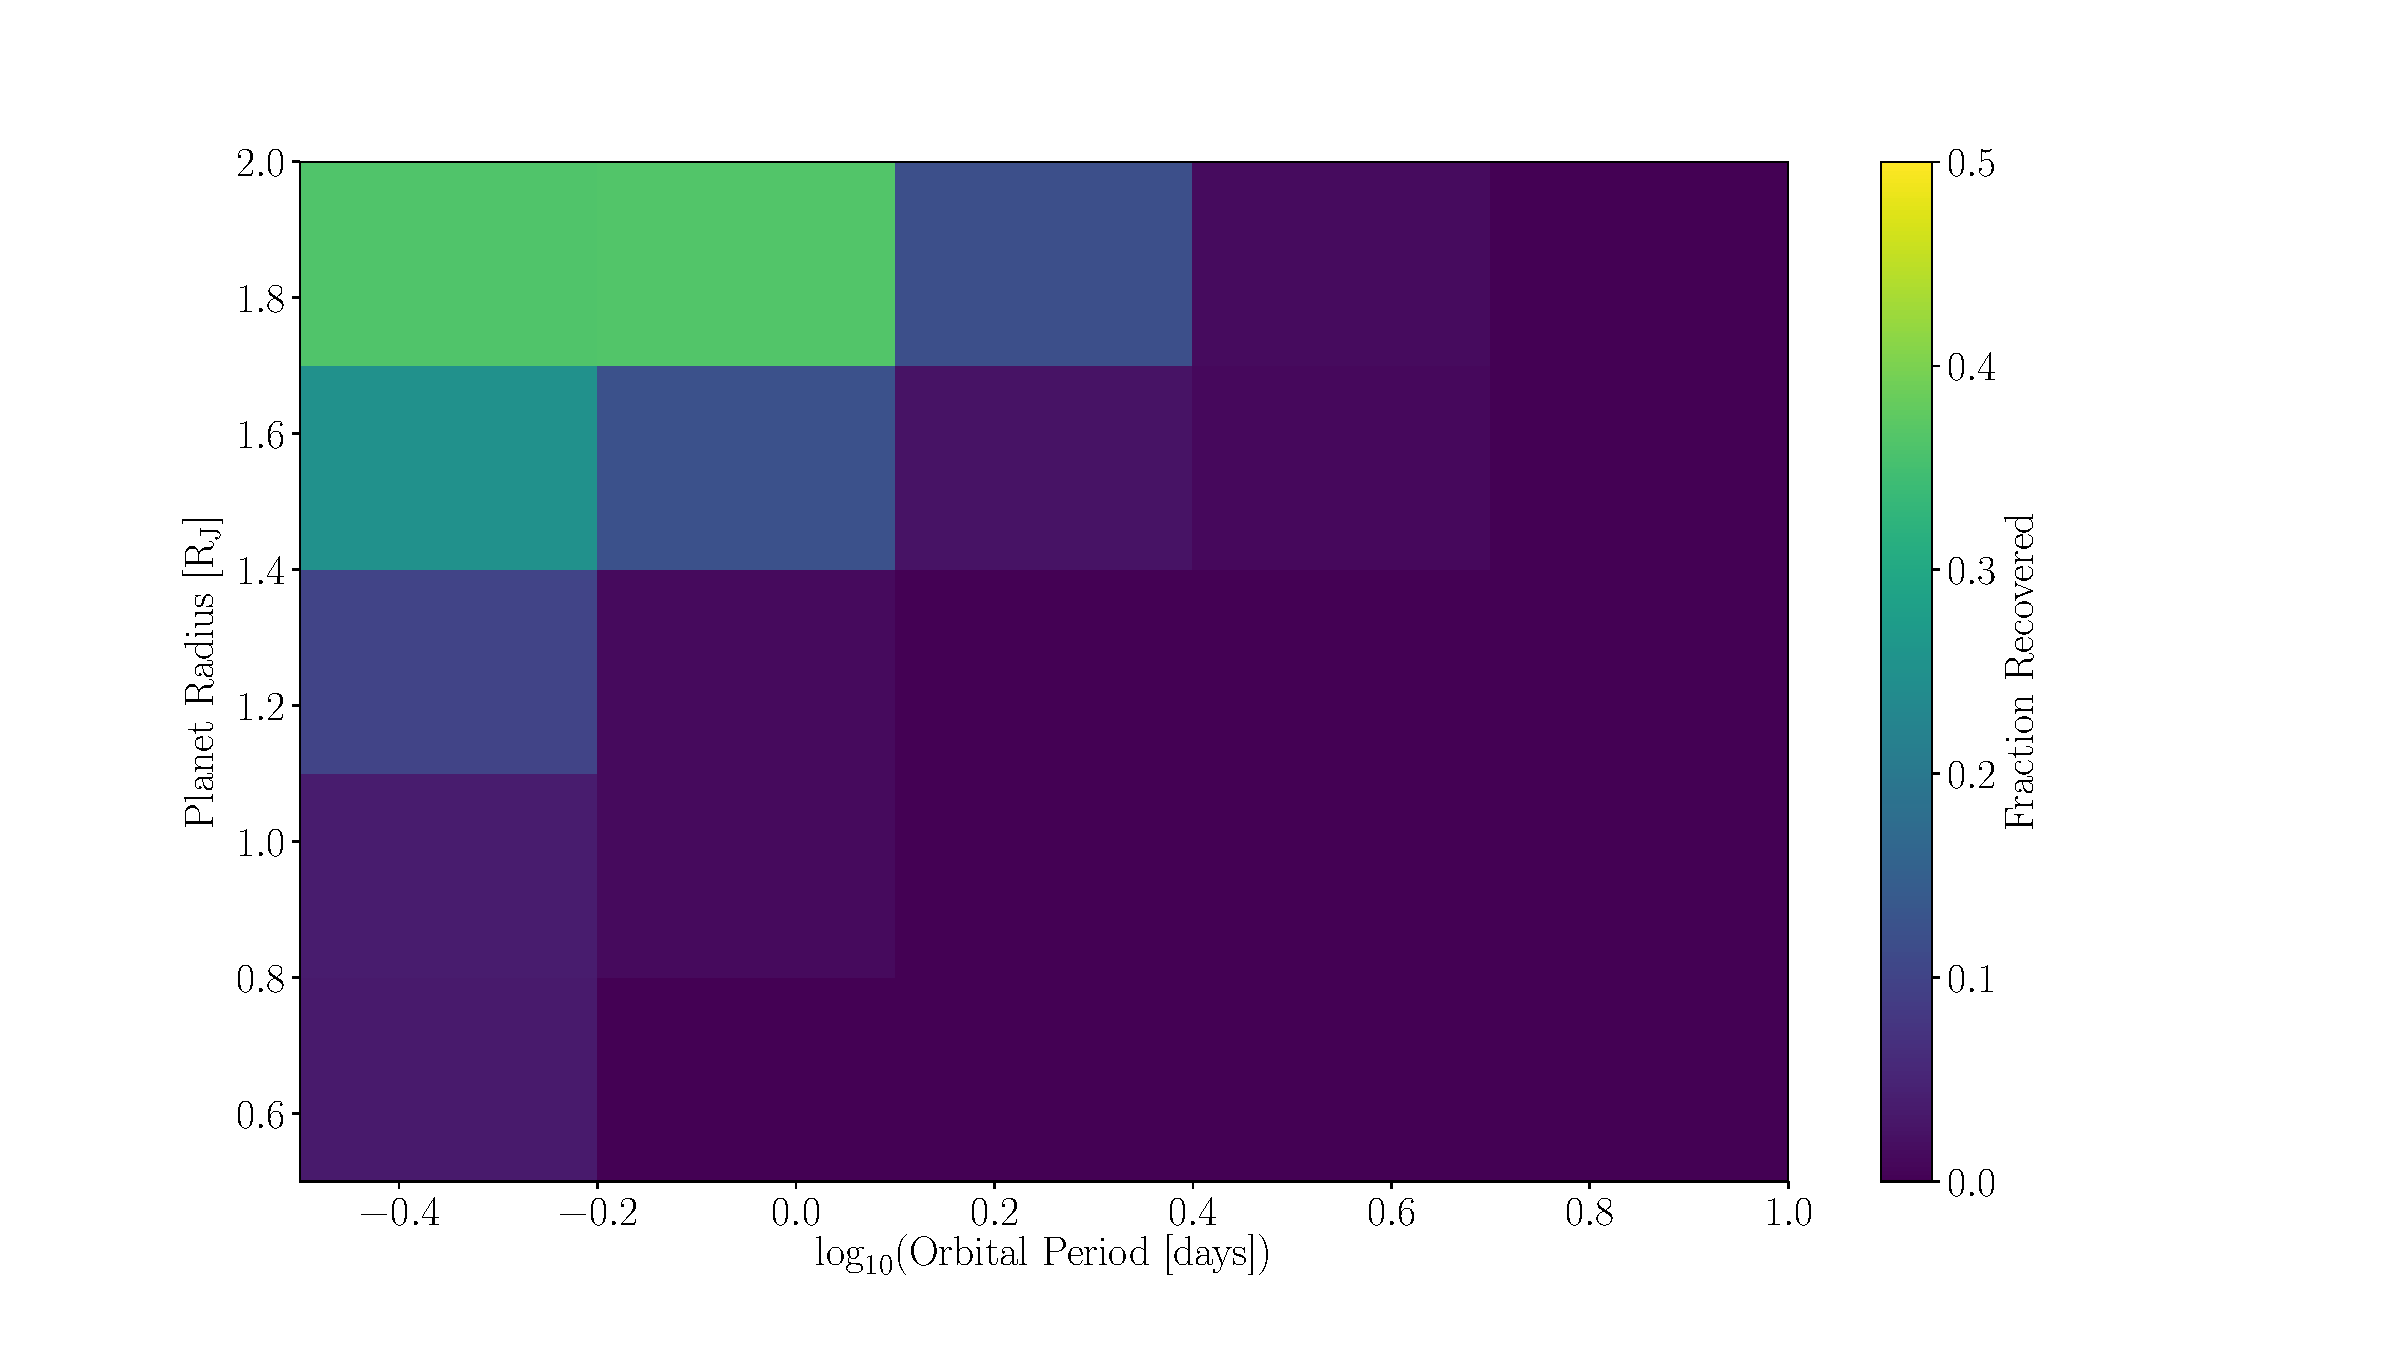
\includegraphics[width=1\textwidth]{completeness.pdf}
\label{fig:completeness}
\end{figure}

% %   - Optimizing cadence and observing strategy
% % We tested a range of cadences by injecting planets into light curves with
% % different cadences and corresponding white noise amplitudes and running BLS on
% % these light curves.
% We simulated DECam light curves with a range of cadences and corresponding
% white noise amplitudes.
% We tested cadences of 3, 5, 8 and 10 minutes with SNRs of 7.0\%, 5.3\%, 4.2\%
% and 3.8\% respectively and found that the most rapid cadence, 3 minute
% integrations, resulted in the largest number of successfully detected
% exoplanets by a marginal amount, despite having the worst photometric
% precision per exposure.
% We also tested a range of observing strategies.
% We simulated light curves for 2 sets of 9 consecutive nights separated by a
% lunar month and 4 sets of 9 nights where observations are conducted
% every-other-night, separated by a lunar month.
% We found that closely spacing nights of observations resulted in a slightly
% larger overall number of recovered planets, with slightly more small planets.
% Spreading the same number of nights over a longer baseline with gaps in
% between resulted in slightly better recovery of planets on longer orbital
% periods, although a smaller number of planets were recovered overall.
% % Since our sensitivity to planet transits rapidly decreases with increasing
% % orbital period, and our planet detection pipeline we structure our observing strategy

% found that targeting the
% L \& SMC over multiple series of consecutive nights resulted in a greater number
% of detected exoplanets than spreading the same number of nights over a longer
% time baseline.

% Results
%   - Prospects: yields and predictions

% Discussion & Conclusion
%   - Caveats and challenges
There are some caveats and limitations to the simulations conducted here.
Firstly, we only included white noise in our simulated light curves, however
time series photometry obtained from the DECam is likely to have correlated
noise due to changes in the point spread function as the instruments flex with
shifting attitude, temperature and pressure.
In addition, planet transits and eclipses may be superposed on time-variable
signals from the host star due to its rotation.
Another caveat to this study is that we only simulated transit signals with
zero impact parameter, \ie\ planets transit across the center of the star and
have the longest duration (and deepest) possible transit.
Finally, we did not convolve transit light curves with the integration window.
Transit features are therefore sharper (and easier to detect) than they would
be in a realistic survey.

%   - Implications
% These simulations indicate that we will be able to detect small stars or giant
% planets orbiting Sun-like stars with Large and Small Magellanic clouds.
